%This is a LaTeX template for homework assignments
\documentclass{article}

\usepackage[utf8]{inputenc}
\usepackage{amsmath}
\usepackage{amssymb}
\usepackage{graphicx}
\usepackage{enumitem}

\begin{document}

%\title{EMET1001: ASSIGNMENT WEEK 2}
%\author{ZEMING WANG - U6114134}


%\maketitle
%\vspace{1in}

%TUTOR: LONG

\thispagestyle{empty}

\begin{center}
\huge
\vspace*{1.0in} EMET1001 
\\\vspace{0.5in} ASSIGNMENT 5
\normalsize
\\\vspace{0.5in} \textsc{By}
\\\vspace{0.1in} \textsc{Zeming Wang}
\\\vspace{0.1in} \textsc{u6114134}
\normalsize
\\\vspace{0.5in} \textsc{Tutorial: Thur. 2-3 pm}
\\\vspace{0.1in} \textsc{Tutor: Long}
\normalsize
\\\vspace{0.5in} \textsc{Due: Aug. 22, 2016}
\end{center}

\newpage
\setcounter{page}{1}

\begin{enumerate}
    
    \item[1.] Let $$ f(x) = \frac{ x^2 }{ x^2 + 2 } $$
    
        \begin{enumerate}
            \item[(a)] Compute $f'(x)$ and determine where $f(x)$ is increasing/decreasing.
            
            $$ f'(x) = \frac{ 2x \cdot (x^2+2) - x^2 \cdot 2x }{ (x^2+2)^2 } = \frac{ 4x }{ (x^2+2)^2 } $$
            
            Since $(x^2+2)^2 > 0$ for all $x$, $f'(x)=0 \Leftrightarrow x=0 $.
            
            Therefore, $x=0$ is the stationary point for $f(x)$. \\
            
            When $x>0$, $f'(x)>0$, thus $f(x)$ is increasing.\\
            When $x<0$, $f'(x)<0$, thus $f(x)$ is decreasing. \\
            
            \item[(b)] Find possible inflection points.
            
            $$ f''(x) = \frac{ 4(x^2+2)^2 - 4x \cdot 2(x^2+2) \cdot 2x }{ (x^2+2)^4 } = \frac{ 8-12x^2 }{ (x^2+2)^3 } $$
            
            Let $f''(x) = 0$. Since the denominator is always positive, we have:
            $$  8-12x^2 = 0 \Leftrightarrow x^2 = \frac{2}{3} \Leftrightarrow x = \pm\sqrt{\frac{2}{3}} $$
            
            The possible inflection points are $x = \pm\sqrt{\dfrac{2}{3}}$.
            
            \item[(c)] Determine the limit of $f(x)$ as $x \rightarrow \pm\infty$, and sketch the graph of $f(x)$.
            
            $$ \lim_{x \rightarrow \infty}{f(x)} = \lim_{x \rightarrow \infty}{ \frac{x^2}{x^2+2} } 
               = \lim_{x \rightarrow \infty}{ \frac{1}{1+\frac{2}{x^2}} } = 1 $$
               
            Similarly, we can find:
            $$ \lim_{x \rightarrow -\infty}{f(x)} = 1 $$
            
            Summarize everything we know about $f(x)$:
            \begin{itemize}
                \item $f(x=0) = 0$
                \item $f(x)$ approaches $1$ when $x \rightarrow \pm\infty$
                \item $f(x)$ is decreasing when $x<0$ and increasing when $x>0$
                \item $f(x)$ is convex when $-\sqrt{\frac{2}{3}}<x<\sqrt{\frac{2}{3}}$ and concave when $x<-\sqrt{\frac{2}{3}}$ or $x>\sqrt{\frac{2}{3}}$
            \end{itemize}
            
            Consider all these together, we can sketch the graph of $f(x)$ like this:\\
            
            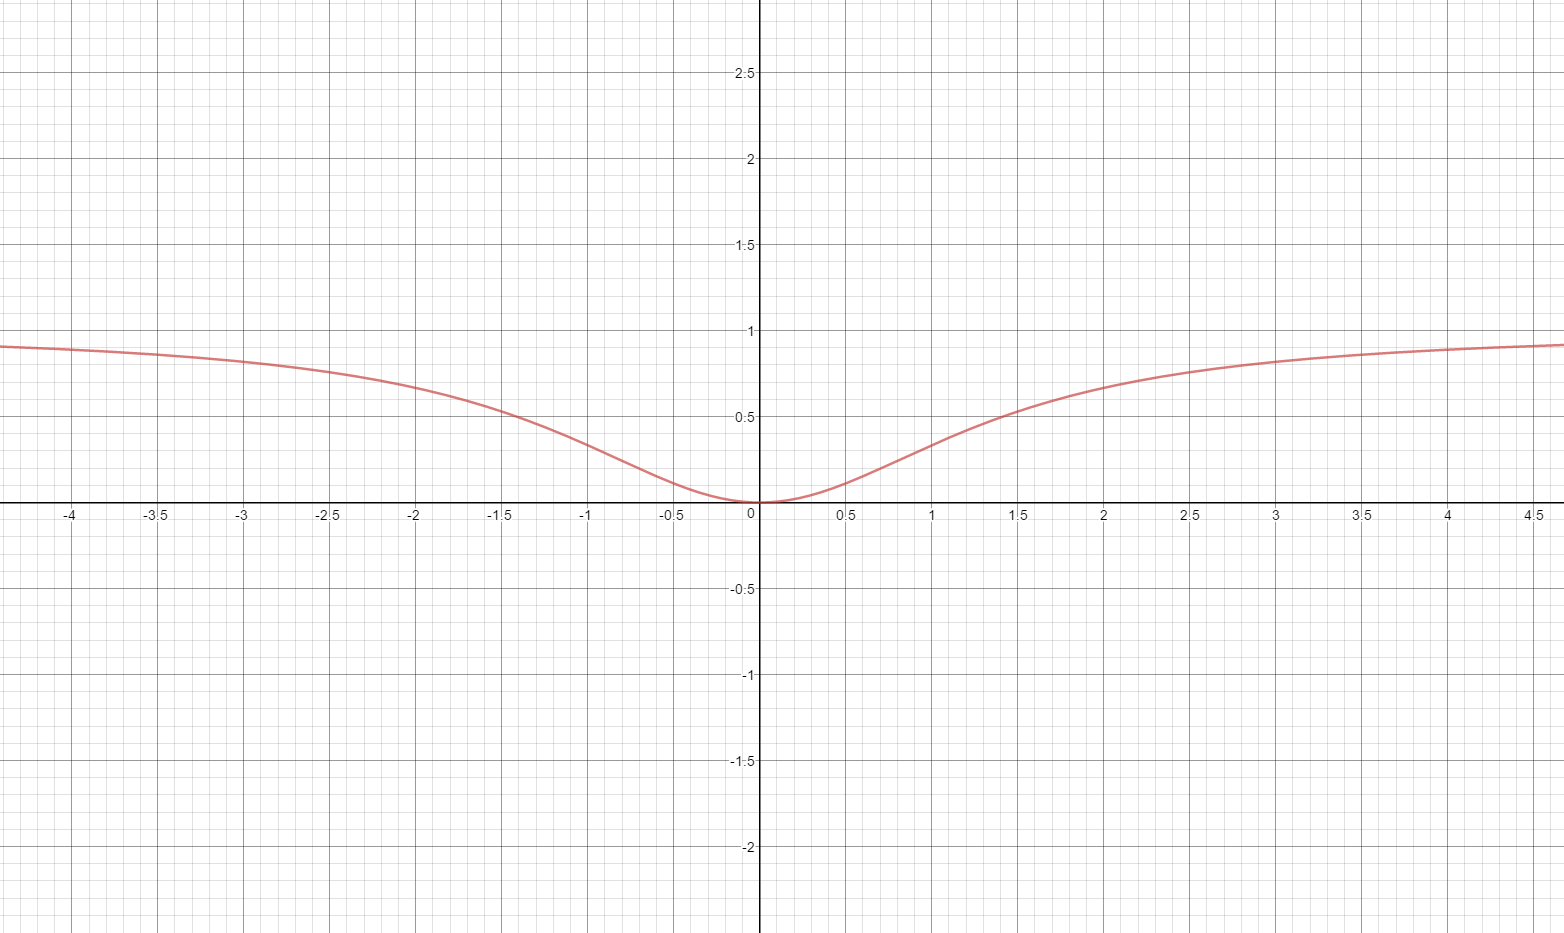
\includegraphics[scale=0.2]{figure_1}
           
        \end{enumerate}
    
    \item[2.] A firm's production function is $Q(L) = 12L^2 - \dfrac{L^3}{20}$, where $L \in [0, 200]$
        \begin{enumerate}
            \item[(a)] Find $L^{*}$ that maximizes $Q(L)$, and $L^{**}$ that maximizes $\dfrac{Q(L)}{L}$.
            
            $$ Q'(L) = 24L - \frac{3L^2}{20} $$
            
            Stationary points found at:
            $$ Q'(L) = 24L - \frac{3L^2}{20} = 0 \implies L=0,\ \textrm{or}\ L=160 $$
            
            So the maximum can be found at either the stationary points or the end points of the interval:
            $$ L_1 = 0, L_2 = 160, L_3 = 200 $$
            
            We can test the value of $Q(L)$ at each of these three points:
            $$ Q(L=0) = 0,\ Q(L=160) = 102400,\ Q(L=200)=80000 $$
            
            Therefore, $ L^{*} = 160 $. \\\\
            
            Let $ R(L) = \dfrac{Q(L)}{L} = 12L - \dfrac{L^2}{20} $. Take derivative of $R(L)$:
            $$ R'(L) = 12 - \frac{L}{10} $$
            
            Stationary points are:
            $$  R'(L) = 12 - \frac{L}{10} = 0 \implies L = 120 $$
            
            By checking the value of $R(L)$ at both the stationary points and the end points, we can confirm that $R(L)$ is maximized when $L=120$. \\
            
            Therefore, $ L^{**} = 120 $. \\
            
        \end{enumerate}
    
    
    \item[6.] Let $g(x) = x - 2\ln{(x+1)}$.
        \begin{enumerate}
            \item[(a)] Where is $g$ defined? \\
            
            $g$ is defined when $x+1>0 \implies x>-1$. \\
            
            \item[(b)] Find $g'(x)$ and $g''(x)$.
            
            $$ g'(x) = 1 - \frac{2}{x+1} $$
            $$ g''(x) = \frac{2}{(x+1)^2} $$
            
            \item[(c)] Find possible extreme points and inflection points. Sketch the graph.
            
            $$ g'(x) = 1 - \frac{2}{x+1} = 0 \implies x = 1 $$
            
            Since  $(x+1)^2>0$ always holds on $(-1,\infty)$, $g''(x)>0$ always holds, which means the graph is convex on the whole domain, there is no inflection point. \\\\
            
            We know:
            
            \begin{itemize}
                \item $g(x=0)=0$
                \item $g'(x)<0$ when $x<1$, and $g'(x)>0$ when $x>1$
                \item $g''(x)>0$ for all $x$ in domain
                \item $\lim_{x \rightarrow -1^{+}}{g(x)} = \infty$ and $\lim_{x \rightarrow \infty} = \infty$
            \end{itemize}
            
            $$$$ The graph is sketched as below: \\
            
            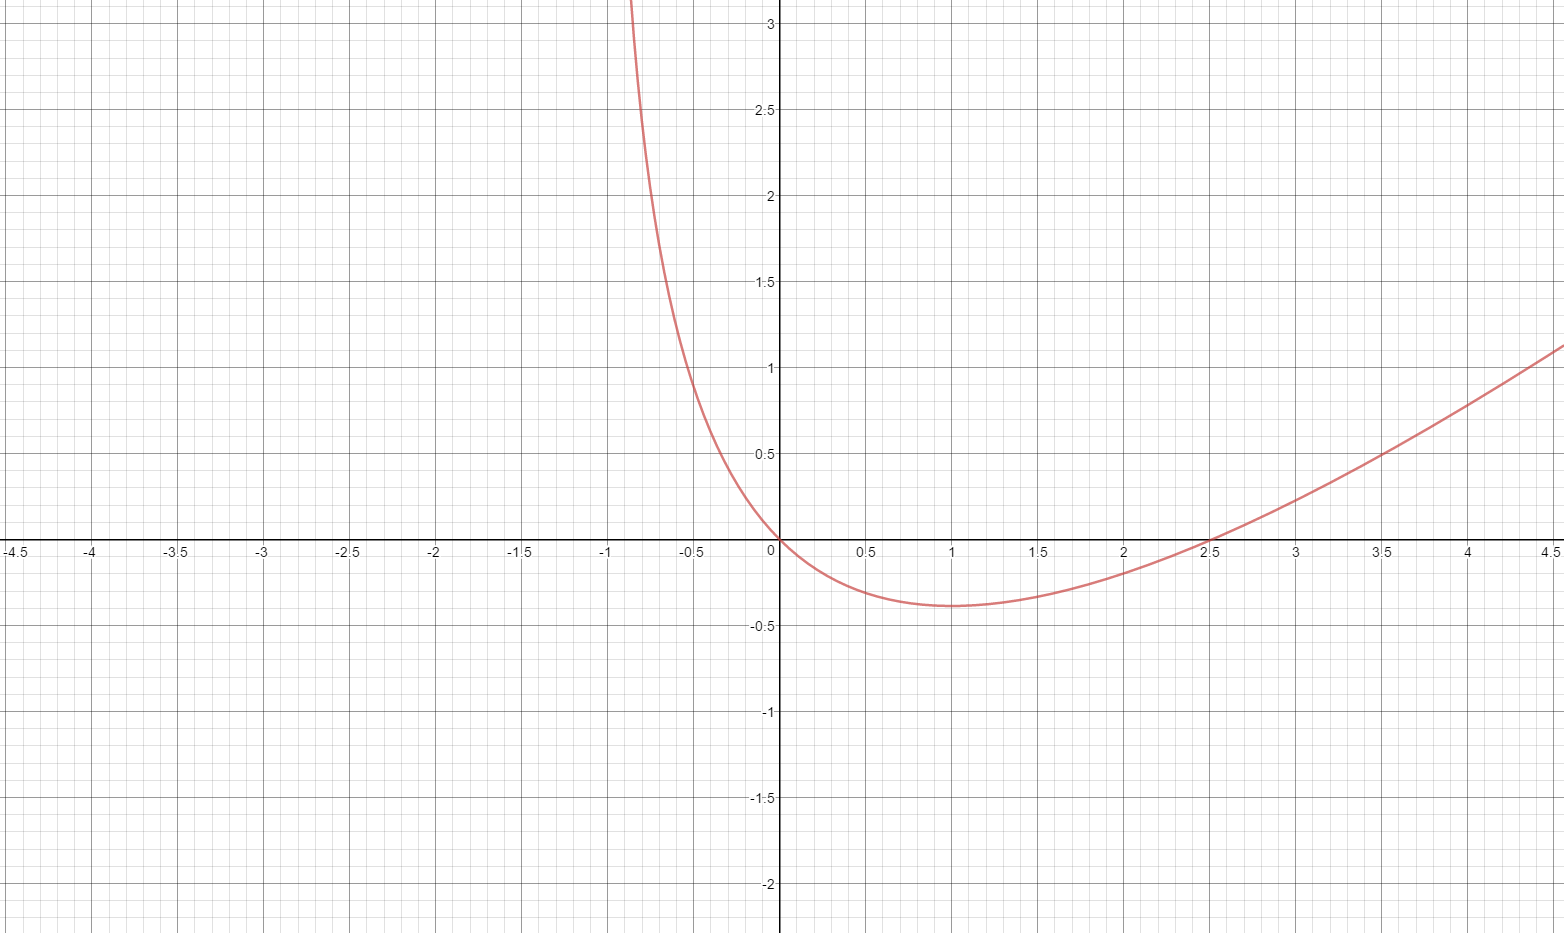
\includegraphics[scale=0.2]{figure_2}
            
        \end{enumerate}
        
    \item[7. ] Let $f(x) = \ln{(x+1)} - x + \dfrac{x^2}{2} - \dfrac{x^3}{6}$
        \begin{enumerate}
            \item[(a)] Find the domain $D_f$ and prove $f'(x) = \dfrac{x^2-x^3}{2(x+1)}$. \\
            
            The only restrain is $x + 1>0$. So the domain $D_f = \{x: x>-1\}$.
            
            $$ f'(x) = \frac{1}{x+1} - 1 + x - \frac{x^2}{2} = \frac{x^2-x^3}{2(x+1)} $$
            
            \item[(b)] Find possible extreme points and inflection points.
            
            $$ f'(x) = \frac{x^2-x^3}{2(x+1)} = 0 \implies x^2-x^3=0 \implies x^2(1-x)=0 \implies x=0,\ \textrm{or}\ x=1 $$
            
            Therefore the possible extreme points are $x=0$, $x=1$. 
            
            $$ f''(x) = \frac{ (2x-2x^2) \cdot 2(x+1) - 2(x^2 - x^3) }{ 4(x+1)^2 } = -\frac{ x^3+x^2-x }{ (x+1)^2 }$$
            
            \begin{equation*}
            \begin{aligned}
                f''(x) = 0 
                &\implies x^3+x^2-x=0 \implies x(x^2+x-1)=0 \\
                &\implies x=0,\ \textrm{or}\ x=\frac{-1+\sqrt{5}}{2}\ (x=\frac{-1-\sqrt{5}}{2} \notin D_f)
            \end{aligned}
            \end{equation*}
  
            Therefore the possible inflection points are $x=0$, $x=\frac{-1+\sqrt{5}}{2}$.\\
            
            \item[(c)] Check $f(x)$ as $x \rightarrow (-1)^+$, and sketch the graph on $(-1,2]$.
            
            $$ \lim_{x \rightarrow (-1)^+}{f(x)} = \lim_{x \rightarrow (-1)^+}{ \ln{(x+1)} - x + \frac{x^2}{2} - \frac{x^3}{6} } = -\infty $$
            
            $$$$ The graph is sketched as below:\\
            
            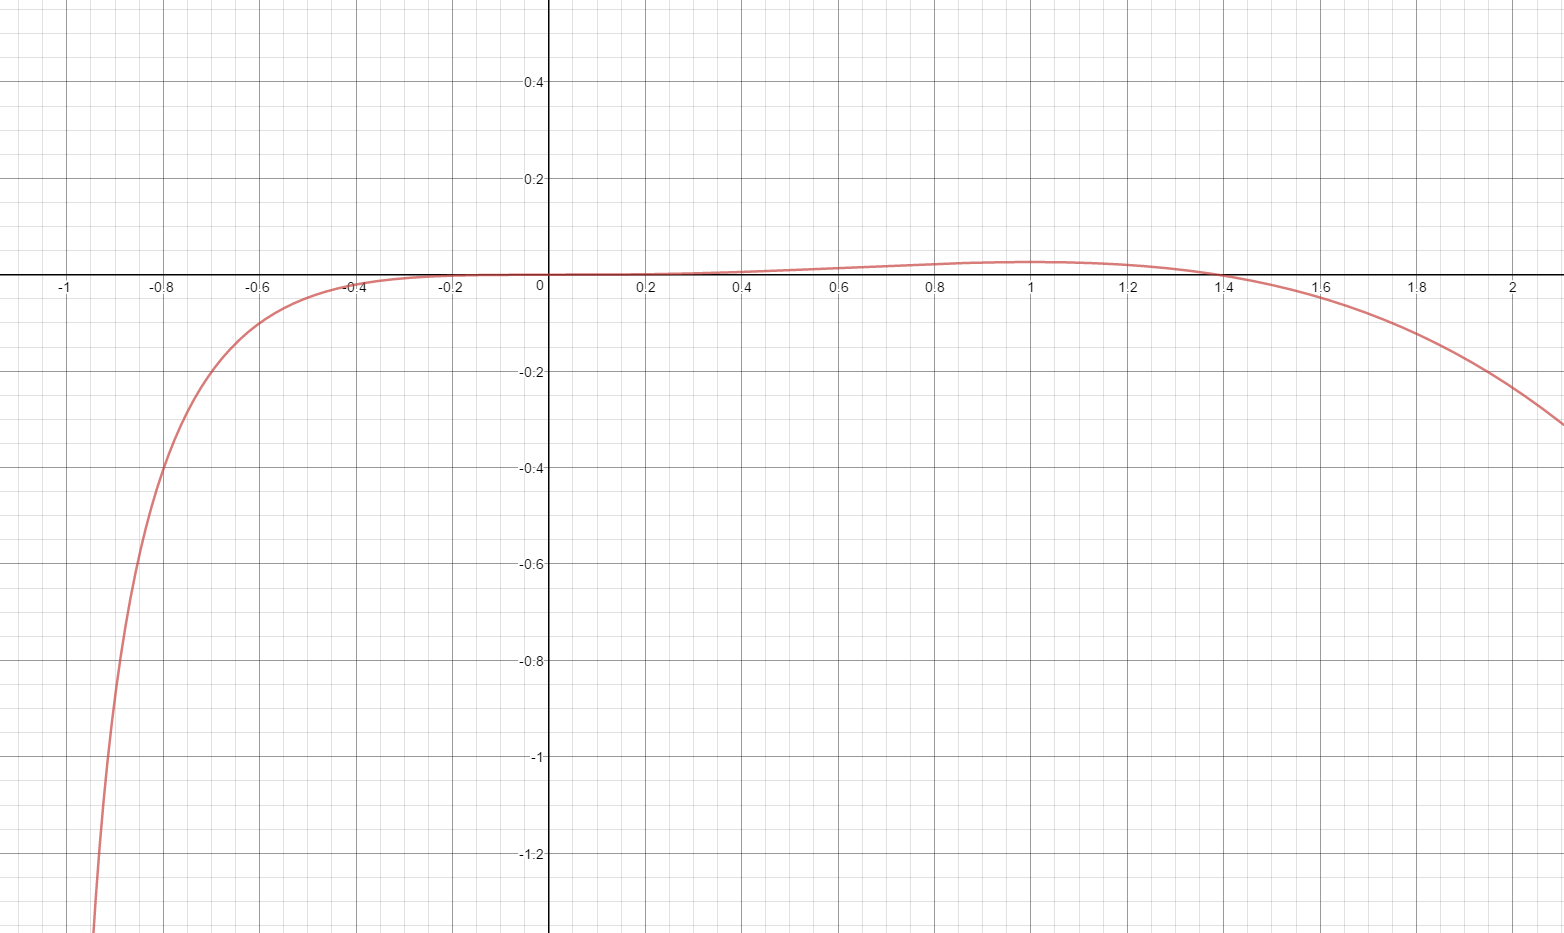
\includegraphics[scale=0.2]{figure_3}
            
        \end{enumerate}
    
    
    \item[8. ] Consider the function $h$ defined for all $x$ by $h(x) = \dfrac{e^x}{1+e^{2x}}$
        \begin{enumerate}
            \item[(a)] Where is $h$ increasing/decreasing? Find possible maximum and minimum points for $h$.
            
            $$ h'(x) = \frac{ e^x \cdot (1+e^{2x}) - e^x \cdot 2e^{2x} }{ (1+e^{2x})^2 } = \frac{ e^x(2-e^{2x}) }{ (1+e^{2x})^2 } $$
            
            Stationary points can be found at:
            $$ h'(x)=0 \implies e^x(2-e^{2x})=0 \implies e^{2x}=2 \implies 2x = \ln{2} \implies x = \ln{\sqrt{2}} $$
            
            When $x<\ln{\sqrt{2}}$, $h'(x)>0$, $h(x)$ is increasing.\\
            When $x>\ln{\sqrt{2}}$, $h'(x)<0$, $h(x)$ is decreasing.\\
            
            So $ x = \ln{\sqrt{2}} $ is the maximum point.\\
            
            \item[(b)] Why does $h$ defined on $(-\infty, 0]$ have an inverse? Find an expression for the inverse function. \\
            
            We know from solution (a) that $h(x)>0$ when $x<\ln{\sqrt{2}}$. Thus $h(x)$ is strictly increasing on $(-\infty, 0]$. \\
            
            We also know that strictly increasing functions are one-to-one. Thus $h(x)$ has an inverse on $(-\infty, 0]$. \\
            
            To find the inverse function, let $y=h(x)$. $y$ reaches its maximum at $x=0$, the end of the interval. The max value is $h(0) = \frac{1}{3}$.
            $$ \lim_{x \rightarrow -\infty}{ \frac{e^x}{1+e^{2x}} } 
              = \lim_{x \rightarrow -\infty}{ \frac{1}{\frac{1}{e^x}+e^x} } = 0 $$
            
            Thus for $x \in (-\infty, 0]$:
            $$ 0 < y \leq \frac{1}{3} $$
            
            Let $z=e^x$. Thus $z \in (0, 1]$.\\
            
            Substitute $e^x$ in the function by $z$:
            $$ y = \frac{z}{2 + z^2} $$
            
            Rearrange the equation:
            $$ z^2 - \frac{1}{y}z + 2 = 0$$
            
            Solve the equation for $z$:
            $$ z = \frac{ \frac{1}{y} \pm \sqrt{\frac{1}{y^2}-8} }{2} $$
            
            We know $y\leq \frac{1}{3}$, therefore,
            $$ z = \frac{ \frac{1}{y} + \sqrt{\frac{1}{y^2}-8} }{2} \geq \frac{\frac{1}{y}}{2} \geq \frac{3}{2} > 1 $$
            is not in the range $(0, 1]$ and thus omitted. \\
            
            While, on the other hand, we have:
            $$ \frac{1}{y} \geq 3 \Leftrightarrow -\frac{4}{y}+4 \leq -8 $$
            
            So we can prove:
            $$ \sqrt{\frac{1}{y^2}-8} \geq \sqrt{ \frac{1}{y^2}-\frac{4}{y}+4 } = 
               \sqrt{ \Bigg( \frac{1}{y}-2 \Bigg)^2 } = \frac{1}{y} - 2 $$
               
            Therefore,
            $$ \frac{1}{y} - \sqrt{\frac{1}{y^2}-8} \leq 2  $$
            
            which means
            $$  z = \frac{ \frac{1}{y} - \sqrt{\frac{1}{y^2}-8} }{2} \leq 1 $$
            is within the range $(0, 1]$ and thus valid. \\
            
            Substitute $z=e^x$ back:
            $$ e^x = \frac{ \frac{1}{y} - \sqrt{\frac{1}{y^2}-8} }{2} $$
            
            Therefore,
            $$ x = \ln{ \frac{ \frac{1}{y} - \sqrt{\frac{1}{y^2}-8} }{2} } = \ln{ \Bigg( \frac{1}{y} - \sqrt{\frac{1}{y^2}-8} \Bigg) } - \ln{2} $$
            
            The inverse function is:
            $$ f^{-1}(x) =\ln{ \Bigg( \frac{1}{x} - \sqrt{\frac{1}{x^2}-8} \Bigg) } - \ln{2},\ \textrm{where}\ x \in (0, \frac{1}{3}] $$
            
        \end{enumerate}
        
\end{enumerate}

\end{document}